\documentclass[../../main.tex]{subfiles}

Der Fragenkatalog besteht aus folgenden Fragen:
\begin{enumerate}
    \item Was ist dein Lieblings-Videospliel?
    \item Lieber Single- oder Multiplayer?
    \item Was ist dein Lieblingsgenre?
    \item Was ist deine Lieblingskonsole?
    \item Was ist dein Lieblings-Free-To-Play Spiel?
    \item Eigene Konsole mitnehmen / zur Verfügung gestellte verwenden?
    \item Welches Spiel hast du in Quarantäne am meißten gespielt?
    \item Hast du in Quarantäne mehr Single- oder Multiplayerspiele gespielt?
    \item Wie wichtig sind dir Videospiele?
\end{enumerate}

\begin{tikzpicture}
    \begin{axis}[
        title={Was ist dein lieblings-Videospiel},
        symbolic x coords={
            Among Us,
            Fortnite,
            COD BO4,
            Detroit,
            GTA V,
            LOL,
            Minecraft
        },
        ybar,
        ylabel={Antwortrate [\%]},
        width=\textwidth,
        height=0.45\textheight,
        xtick=data,
        x tick label style={rotate=45,anchor=east},
    ]
        \addplot+[ybar] plot coordinates {
            (Among Us,10)
            (Fortnite,16)
            (COD BO4,5)
            (Detroit,5)
            (GTA V,5)
            (LOL,5)
            (Minecraft,15)
        };
    \end{axis}
\end{tikzpicture}

\begin{tikzpicture}
    \begin{axis}[
        title={Lieber Single- oder Multiplayer?},
        symbolic x coords={
            Singleplayer,
            Multiplayer
        },
        ybar,
        ylabel={Antwortrate [\%]},
        width=\textwidth,
        height=0.45\textheight,
        xtick=data,
        x tick label style={rotate=45,anchor=east},
    ]
        \addplot+[ybar] plot coordinates {
            (Singleplayer,26)
            (Multiplayer,7)
        };
    \end{axis}
\end{tikzpicture}

\begin{tikzpicture}
    \begin{axis}[
        title={TITLE},
        symbolic x coords={
            a
        },
        ybar,
        ylabel={Antwortrate [\%]},
        width=\textwidth,
        height=0.45\textheight,
        xtick=data,
        x tick label style={rotate=45,anchor=east},
    ]
        \addplot+[ybar] plot coordinates {
            
        };
    \end{axis}
\end{tikzpicture}

\begin{tikzpicture}
    \begin{axis}[
        title={TITLE},
        symbolic x coords={
            a
        },
        ybar,
        ylabel={Antwortrate [\%]},
        width=\textwidth,
        height=0.45\textheight,
        xtick=data,
        x tick label style={rotate=45,anchor=east},
    ]
        \addplot+[ybar] plot coordinates {
            
        };
    \end{axis}
\end{tikzpicture}

\begin{tikzpicture}
    \begin{axis}[
        title={TITLE},
        symbolic x coords={
            a
        },
        ybar,
        ylabel={Antwortrate [\%]},
        width=\textwidth,
        height=0.45\textheight,
        xtick=data,
        x tick label style={rotate=45,anchor=east},
    ]
        \addplot+[ybar] plot coordinates {
            
        };
    \end{axis}
\end{tikzpicture}

\begin{tikzpicture}
    \begin{axis}[
        title={TITLE},
        symbolic x coords={
            a
        },
        ybar,
        ylabel={Antwortrate [\%]},
        width=\textwidth,
        height=0.45\textheight,
        xtick=data,
        x tick label style={rotate=45,anchor=east},
    ]
        \addplot+[ybar] plot coordinates {
            
        };
    \end{axis}
\end{tikzpicture}

\begin{tikzpicture}
    \begin{axis}[
        title={TITLE},
        symbolic x coords={
            a
        },
        ybar,
        ylabel={Antwortrate [\%]},
        width=\textwidth,
        height=0.45\textheight,
        xtick=data,
        x tick label style={rotate=45,anchor=east},
    ]
        \addplot+[ybar] plot coordinates {
            
        };
    \end{axis}
\end{tikzpicture}

\begin{tikzpicture}
    \begin{axis}[
        title={TITLE},
        symbolic x coords={
            a
        },
        ybar,
        ylabel={Antwortrate [\%]},
        width=\textwidth,
        height=0.45\textheight,
        xtick=data,
        x tick label style={rotate=45,anchor=east},
    ]
        \addplot+[ybar] plot coordinates {
            
        };
    \end{axis}
\end{tikzpicture}

\begin{tikzpicture}
    \begin{axis}[
        title={TITLE},
        symbolic x coords={
            a
        },
        ybar,
        ylabel={Antwortrate [\%]},
        width=\textwidth,
        height=0.45\textheight,
        xtick=data,
        x tick label style={rotate=45,anchor=east},
    ]
        \addplot+[ybar] plot coordinates {
            
        };
    \end{axis}
\end{tikzpicture}

\begin{tikzpicture}
    \begin{axis}[
        title={TITLE},
        symbolic x coords={
            a
        },
        ybar,
        ylabel={Antwortrate [\%]},
        width=\textwidth,
        height=0.45\textheight,
        xtick=data,
        x tick label style={rotate=45,anchor=east},
    ]
        \addplot+[ybar] plot coordinates {
            
        };
    \end{axis}
\end{tikzpicture}